\documentclass[11pt]{article}

\usepackage{maiacustom}

\begin{document}

\psettitle{Banco de questões de astronomia}

Estas questões foram produzidas/selecionadas cuidadosamente com o objetivo de preparar os estudantes para o processo seletivo de astronomia no Brasil. Algumas questões não são de autoria própria e estão devidamente sinalizadas por () antes do enunciado. O template do banco de questões é o mesmo do Professor \text{Kevin Zhou}. Seu trabalho é valioso, e diversas ideias desta lista podem ser encontradas em seus Handouts.

% \begin{psidea}{Título da Ideia}{}
% Ideia
% \end{psidea}

% \begin{psexample}{Título do Exemplo}{}
% Exemplo
% \end{psexample}

% \begin{pssolution*}{}{}
% Solução
% \end{pssolution*}

% \begin{psremark*}{Título da Observação}{}
% Observação
% \end{psremark*} 
\section{Fotometria e Física Moderna}

\pts{3} 
\begin{pproblem}
    O objetivo dessa questão é deduzir uma expressão para a \textit{profundidade óptica}. Imagine que um feixe de luz passe por uma região do espaço, com uma determiada quantidade de partículas. Se \(I_0\) é a intensidade da luz antes de passar por tal região de espaço e \(I\) é a intensidade da luz após, a profundidade óptica é definida como:
    \[I = I_0e^{-\tau}\]
    Onde \(\tau\) é a profundidade óptica.
    \\
    Considere uma região do espaço possuí densidade numérica de partículas \(n\).
    \begin{alternativas}
        \item Qual o número de partículas em uma área \(A\) e espessura \(dz\)?
        \item Supondo que cada partícula possua sessão transversal \(\sigma\), qual é a área tampada pelas parículas?
        \item Encontre a fórmula para \(\tau\). 
    \end{alternativas}

\begin{pssolution*}{}{}
    \begin{alternativas}
        \item A densidade volumétrica de partículas é \(n\), sendo assim temos que o número \(dN\) de partículas em um volume \(dV\) é dado por
        \[\boxed{dN = ndV \equiv nAdz}\]

        \item Se cada particula ocupa uma área \(\sigma\), a área ocupada por \(dN\) particulas é
        \[\boxed{dS = \sigma dN = \sigma nAdz}\]

        \item É esperado que a área ocupadas pelas particulas seja um empecilho para a passagem da luz. Como a Intensidade é proporcional a área disponível para a passagem da luz, nós temos
        \[\frac{dI}{I} = -\frac{dS}{A} = -n\sigma dz\]
        Integrando, obtemos

        \[I = I_0 e^{-n\sigma z}\]

        Ou seja, 

        \[\boxed{\tau = n\sigma z}\]
    \end{alternativas}
\end{pssolution*}
\end{pproblem}

\pts{2}
\begin{pproblem} A Galáxia do Triângulo, \(M33\), é a terceira maior galáxia do grupo local, ela está a uma distância \(d=970 \text{ kpc}\) de nós e possuí magnitude aparente de \(5,72\). Sabendo que ela possuí aproximadamente \(40\) bilhões de estrelas, encontre a luminosidade média das estrelas de \(M33\). Sua estimativa parece condizer com a realidade? Por que?
\begin{pssolution*}{}{}
    Utilizando a equação de Pogson

    \[m-M_\odot = -2,5\log \left(\frac{L_{g}}{L_\odot}\left(\frac{10 \text{ pc}}{d}\right)^2\right)\]

    Resolendo para \(L_g\), 

    \[L_g = L_\odot \left(\frac{d}{10\text{ pc}}\right)^2 10^{-0,4(m-M_\odot)}\]

    Temos também, que \(L_g = \overline{L_\star} N\) e assim

    \[\overline{L_\star} = \frac{L_\odot}{N} \left(\frac{d}{10\text{ pc}}\right)^2 10^{-0,4(m-M_\odot)}\]

    Utilizando os valores da tabela de constantes, obtemos:

    \[\overline{L_\star} \approx 0,1L_\odot\]

    No entando, essa estimativa não condiz com a realidade, uma vez que há fatores como a extinção interestelar que contribuem para o aumento da magnitude aparente de \(M33\), uma estimativa condizente estaria na mesma ordem de grandeza da Luminosidade do Sol.

\end{pssolution*}
\end{pproblem}

\pts{4}
\begin{pproblem}
    Considere que o universo possuí densidade numérica de estrelas, isto é, numero de estrelas por unidade de volume, constante e de valor \(n\). Assumindo que todas elas tenham \(L = L_\odot\) e que existam um total de \(N_0\) estrelas no universo.
    
    \begin{alternativas}
    \item qual a probrabilidade da magnitude absoluta de uma estrela, vista do centro do universo, ter magnitude entre \(m\) e \(m+dm\), onde \(dm\) é uma porção infinitesimal de magnitude? Deixe sua resposta em termos de \(m\) e da maior magnitude possivél, \(m_{lim}\), de uma estrela na "borda" do universo.

    \item Qual a probabilidade de uma estrela poder ser observada a olho nu?
    
    \textbf{Dados:} \[\int_{-\infty}^{6}10^{0,6(x-A)}dx \approx 2881.6 e^{-1.381 A}\]
    \end{alternativas}\begin{pssolution*}{}{}
    \begin{alternativas}
    \item A magnite aparente de uma estrela é dada por, 

    \[m = -2,5\log F + C\]

    Onde \(C\) é uma constante. Escrevendo \(F = L/4\pi r^2\), temos, 

    \[m = -2,5\log\left(\frac{L}{4\pi r^2}\right) + C = 5\log r -2,5 \log \left(\frac{L}{4\pi}\right)+ C\]

    Mas como \(L\) é constante para todas as estrelas, podemos absorver o segundo termo para a constante. Assim, 

    \[m=5\log r + C \rightarrow r = 10^{0,2(m-C)}\]

    Derivando a expressão de \(m\), temos, 

    \[\frac{dm}{dr} = \frac{5}{r\ln 10}\]

    Agora, vamos achar a probabilidade de uma estrela estar a uma distância \(r\).

    O numero de estrelas contidas entre \(r\) e \(r+dr\) é 

    \[dN(r) = 4\pi n r^2dr\]

    Dividindo por \(N_0\), temos que a probabildiade de uma estrela estar nessa distância é 

    \[dP(r) = \frac{dN(r)}{N_0} = \frac{4\pi n r^2}{N_0}dr \rightarrow dr = \frac{N_0}{4\pi n r^2} dP(r)\]

    Substituindo a expressão para \(dr\), 

    \[\frac{r\ln 10}{5}dm = \frac{N_0}{4\pi n r^2}dP(r)\]

    Isolando \(dP(r)\), 

    \[dP(r) = \frac{4\pi \ln 10 n r^3}{5 N_0}dm\]

    Substituindo a expressão de \(r\), podemos realizar a mudança de variável \(r\rightarrow m\)em \(dP\)

    \[dP(m) = \frac{4\pi n \ln 10  }{5 N_0}10^{0,6(m-C)}dm\]

    Para achar o valor de \(C\), vamos comparar com a magnitude limite, na "borda" do universo. Como o universo possuí \(N_0\) estrelas, seu raio deve ser dado por, 

    \[N_0 = \frac{4\pi R^3}{3} \rightarrow R = \left(\frac{3N_0}{4\pi}\right)^{1/3}\]

    Equacionando agora para \(m_{lim}\), 
    
    \[m_{lim} = 5\log R + C\]

    No qual, podemos isolar a constante \(C = m_{lim}-5\log R\). Substituindo na expresssão de \(dP(m)\),

    \[dP(m) = \frac{4\pi n \ln 10  }{5 N_0}10^{0,6(m-m_{lim}+5\log R)}dm\]

    Trabalhando nessa expressão, 

    \[dP(m) = \frac{4\pi n \ln 10  }{5 N_0}10^{0,6(m-m_{lim})}10^{3\log R}dm\]

    Usando as propriedades do log, \(a\log b = \log b^a\) e \(10^{\log x} = x\), temos, 

    \[dP(m) = \frac{4\pi n R^3\ln 10}{5N_0}10^{0,6(m-m_{lim})}dm\]

    Substituindo \(R\), 

    \[\boxed{dP(m) = \frac{3\ln 10}{5}10^{0,6(m-m_{lim})}dm}\]

    Ou seja, a probabilidade não depende de \(n\) e nem de \(N_0\)!

    \item Para uma estrela ser vísivel, sua magnitude deve ser \(m\leq 6\), assim, equacionando, 
    
    \[P(m\leq 6) = \int_{-\infty}^6 dP(m) = \frac{3\ln 10}{5}\int_{-\infty}^610^{0,6(m-m_{lim})}dm\]

    Usando a integral dada no enuncicado, 

    \[P(m\leq 6) = \frac{3\ln 10}{5}2881,6 e^{-1,381 m_{lim}}\]

    Simplificando os fatores numéricos, 

    \[\boxed{P(m\leq 6) \approx 3981,08 e^{-1,381 m_{lim}}} \]

    A fim de curiosidade, colocando \(m_{lim}\approx 40\), para uma estimativa, teriamos, 

    \[P(m\leq 6)\approx 10^{-20}\]

    Ou seja, mesmo no modelo mais simples o universo, a nossa capacidade e insigficicancia prevalece.
    \end{alternativas}

\end{pssolution*}
\end{pproblem}

\pts{4}
\begin{pproblem}
    O \textit{Brilho Superfícial}, fluxo por ângulo sólido por frequência, \(B_\nu\) é dada pela Lei de Plank:
    \[B_\nu = \frac{dF}{d\nu d\Omega} = \frac{2h\nu^3}{c^2(e^{\frac{h\nu}{k_BT}}-1)}\] 
    \begin{alternativas}
        \item Encontre uma expressão para:
        \[B_\lambda = \frac{dF}{d\lambda d\Omega}\]
        \item A partir de \(B_\lambda\) encontre o comprimento de onda máximo de onda \(\lambda_{max}\) que uma estrela de temperatura \(T\) emite (você terá que resolver algo numéricamente).
        \item Para pequenas frequências temos a aproximação de Righlight-Jeans. Obetenha uma expressão para \(B_\nu\) para frequêncais pequenas.
        \end{alternativas}

\begin{pssolution*}{}{}
    \begin{alternativas}
        \item Temos que
        \[B_\lambda = \frac{dF}{d\lambda d\Omega} = \frac{dF}{d\nu d\Omega}\frac{d\nu}{d\lambda}\]

        Utilizando a relação fundamental da ondulatória, \(c=\nu\lambda \rightarrow \nu = c/\lambda\) chegamos em 

        \[B_\lambda = \frac{2h(c/\lambda)^3}{c^2(e^{\frac{hc}{\lambda k_BT}}-1)}\frac{d}{d\lambda}\left(\frac{c}{\lambda}\right) = \frac{2hc^2}{\lambda^5}\frac{1}{(e^{\frac{hc}{\lambda k_BT}}-1)}\]

        \item Para resolver esse item, pracisamos achar o ponto máximo de \(B_\lambda\). Mas diferenciar \(B_\lambda\) diretamente é uma tarefa estremamente chata. Uma ideia mais eficiente é tirar o logaritimo natural de \(B_\lambda\) e diferenciar o mesmo. Uma vez que estamos no ponto de máximo, ambas as maneiras chegarâo no mesmo, resultado
        
        \[\ln B_\lambda = -5\ln \lambda - \ln (e^{hc/\lambda k_BT}-1) + C\]

        Onde \(C\) é uma constante que absorve os \(\ln\) das outras constantes de  \(B_\lambda\). Continuando a derivar 

        \[\frac{d \ln B_\lambda}{d\lambda} = -\frac{5}{\lambda} + \frac{e^{hc/\lambda k_BT}}{e^{hc/\lambda k_BT}-1}\frac{hc}{k_BT\lambda^2}=0\]

        Definindo \(x = \frac{hc}{k_BT\lambda}\) 

        \[\frac{xe^x}{e^x-1}=5\]

        \[x=5e^{-x}(e^x-1) = 5(1-e^{-x})\]

        Utilizando iteração, podemos resolver para \(x\), obtendo \(x\approx 4,965\). Voltando a definição de \(x\)

        \[4,965 = \frac{hc}{k_B T\lambda_{max}}\rightarrow \boxed{\lambda_{max} \approx \frac{2,989 \cdot 10^{-3}}{T}}\]

        Essa é a famosa \textit{Lei de Wien}, comumente escrita na forma \(\lambda = b/T\), onde \(b\approx 2,989 \cdot 10^{-3}\).

    \end{alternativas}
\end{pssolution*}
\end{pproblem}

\pts{3}
\begin{pproblem}
    A luminosidade de um corpo secundário, depende da área iluminada vísivel do astro. Nestá questão vamos fazer um breve estudo sobre esse fenômeno.
    \begin{alternativas}
        \item  Considere a Seguinte situação:
        \begin{figure}[H]
            \centering
            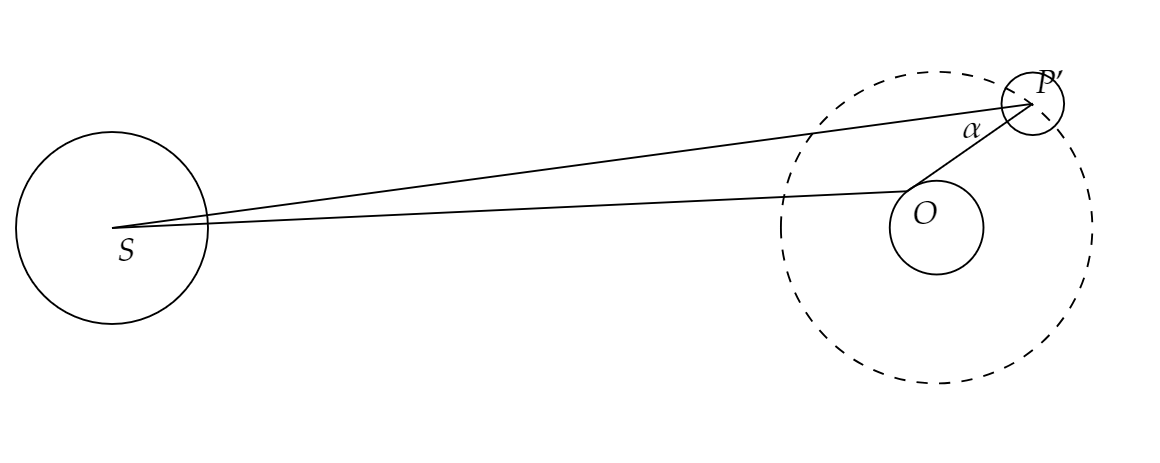
\includegraphics[width=0.8\linewidth]{imagens/fotometria 1.png}
            \caption{Esquema Sol-Terra-Lua}
        \end{figure}

        Encontre uma expressão para a razão \(\Phi\) entre a área iluminada em função de \(\alpha\) e a área total do planeta.
        
        \item Encontre os ângulos \(\alpha\) em que temos a fase da Lua em: Nova, crescente, cheia e minguante, respectivamente.
    \end{alternativas}

\begin{pssolution*}{}{}
    Para resolver a questão, vamos nos guiar no esquema da imagem abaixo:
    \begin{figure}[H]
       \centering
       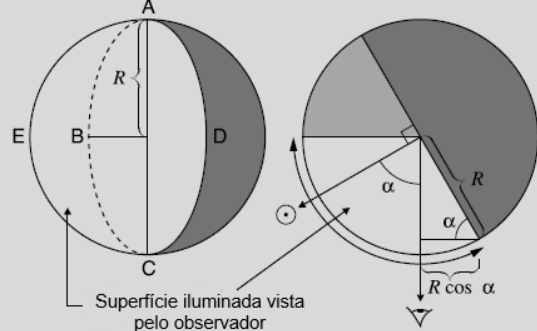
\includegraphics[width=0.8\linewidth]{imagens/fotometriaplanetaria.png}
       \caption{Fonte: Introduction do Planetary Fotometry} 
    \end{figure}

    Do lado esquerdo, vamos um esquema de como o plaeta se parece no céu e na direita uma representação vista "de cima". Aqui, podemos perceber que a área que vemos é composta por metade da área do cículo mais metadade da área de uma elipse de semi eixo maior \(R\) e semi eixo menor \(R\cos\alpha\). Assim

    \[\Phi = \frac{\pi R^2/2 + \pi R^2\cos\alpha/2}{\pi R^2} \ \boxed{\therefore \Phi = \frac{1+\cos\alpha}{2}}\]

    Na Lua nova, temos \(\Phi = 0\), na crescente \(\Phi = 1/2\), na cheia \(\Phi = 1\) e na minguante \(\Phi = 1/2\), assim:

    \[\boxed{\alpha_{nova} = 180^\circ, \ \alpha_{crescente} = 90^\circ, \ \alpha_{cheia} = 0^\circ, \ \alpha_{minguante} = 90^\circ}\]
\end{pssolution*}
\end{pproblem}

\pts{5}
\begin{pproblem} (Apostila Magna)
    Neste problema, modelaremos o efeito da atmosfera na Terra. Suponha que o Sol
seja um corpo negro de temperatura \(T_1\) e raio \(R_1\). A Terra é uma esfera que está localizada
a uma distância \(R\) do Sol e possui raio \(R_3\). A emissividade da Terra é \(\epsilon_3\).
\begin{alternativas}
    \item Se não houvesse atmosfera na Terra, determine sua temperatura de equilíbrio, \(T_3\).
    \item  Agora, consideraremos os efeitos da atmosfera. Modele-a como uma casa esférica de gás,
    com uma emissividade \(\epsilon_2\) e raio exterior \(R_2>R_3\), concêntrica à Terra. No equilíbrio térmico,
    sua absortividade para os comprimentos de onda no ultravioleta e no infravermelho é \(\epsilon_2\). A
    atmosfera transmite uma fração \(t\) da radiação ultravioleta mas é completamente opaca ao
    infravermelho. Assumindo que o Sol emita luz ultravioleta enquanto a Terra emite e re-emite
    no infravermelho, determine as temperaturas \(T_2\) da atmosfera e \(T_3\) da Terra, no equilíbrio
    termodinâmico. Assuma que a atmosfera seja um condutor de calor perfeito, de forma que
    toda a radiação incidente sobre ela seja uniformemente distribuída por sua superfície.
\end{alternativas}

\begin{pssolution*}{}{}
    \begin{alternativas}
        \item No equilíbiro termodinâmico, temos que a quantidade de potencia absorvida é a mesma que a emitida. Além disso, a emissividade e a absortividade são as mesmas. Desse modo, 
        \[\frac{4\pi R_1^2\sigma T_1^4}{4\pi R^2}\pi R_3^2\epsilon_3 = 4\pi R_3^2\sigma T_3^4\epsilon_3\]

        Resolvendo para \(T_3\), 

        \[\boxed{T_3 = T_1\left(\frac{R_1^2}{4\pi R^2}\right)^{1/4}}\]

         \item A temperatura da atmosfera é calculada por 
         
         \[T_2 = T_1\left(\frac{R_1^2}{4\pi R^2 }\right)^{1/4}\]

         O processo é analogo ao item anterior. A luminosidade transmitida pela terra é, 

         \[L_2 = {4\pi R_2^2\sigma T_2^4\epsilon_2} t\]

         A Terra irá refletir toda essa radiação e a atmosfera refletirá de volta apenas uma fração t, desse modo, a luminosidade total é dadda por, 

         \[L_{2,T} = 4\pi R_2^2\sigma T_2^4\epsilon_2 (t+t^2+t^3+...)\]

         O item dentro do parenteses é uma somatóriso de PG infinito, com \(q_1 = t\) e \(r = t\), como \(t<1\), o valor do somatório vale, 

         \[(t+t^2+t^3+...) = \sum_{n=1}^{\infty}t^n = \frac{t}{1-t}\]

         Igualando ambas, 

         \[L_{2,T} = L_3 \rightarrow \frac{4\pi R_2^2\sigma T_2^4 \epsilon_2 t}{1-t} = 4\pi R_3^2\sigma T_3^4\]

         Resolvendo para \(T_3\), 

         \[T_3 = T_2\left(\frac{R_2^2\epsilon_2}{R_3^2}\frac{t}{1-t}\right)^{1/4}\]

         Substituindo o valor de \(T_2\), 

         \[\boxed{T_3 =T_1\left(\frac{R_1^2R_2^2}{4\pi R^2R_3^2}\frac{\epsilon_2t}{1-t}\right)^{1/4}}\]


    \end{alternativas}
    
\end{pssolution*}
\end{pproblem}


\pts{2}
\begin{pproblem}(Lista 2 - 2021)
    A Nebulosa do Anel (M57) possui uma magnitude aparente igual a 9 e um
diâmetro angular de 2$^{\prime}$ para um observador na Terra. Qual seria a magnitude aparente do céu
noturno de um planeta orbitando uma estrela exatamente no centro de M57?
\begin{pssolution*}{}{}
    O céu noturno compreende um ângulo sólido de \(2\pi\) sr, já o ângulo sólido visto por nés é \(\Omega \approx \pi \theta^2\), onde \(\theta\) é o raio angular. Como o Fluxo é proporcional a \(\Omega\), temos

    \[m_{ceu}-m = -2,5\log\left(\frac{\Omega_{ceu}}{\Omega}\right)\]

    Para converter \(\Omega\) de arco-minuto\(^2\) para sr, temos que multiplicar por \(\left(\frac{\pi}{180\cdot60}\right)^2\), assim
    
    \[m_{ceu} = 9 - \log\left(\frac{2\pi}{\pi(\frac{\pi}{180\cdot60})^2}\right)\]

    \[\boxed{m_{ceu} = -9,43}\]
\end{pssolution*}
\end{pproblem}


\pts{4}
\begin{pproblem} (Adaptado Lista 4 - 2021)
    O Efeito Cherenkov foi primeiramente detectado pelo cientista soviético
    Pavel Cherenkov, em 1937. Mais tarde, em conjunto com seus colegas de trabalho, I. E. Tamm e
    I. M. Frank, ele interpretou fisicamente o fenômeno, ganhando, assim, o Prêmio Nobel de Física
    de 1958. Antes de fazer um estudo matemático, precisamos, primeiro, entender um pouco mais
    sobre seu princípio.

    Quando partículas carregadas de alta energia percorrem um meio dielétrico, é possível que, caso
    sua velocidade seja maior que a velocidade de fase ($\frac{c}{n}$), átomos sejam excitados. Esses, por sua
    vez, ao retornarem ao estado fundamental, emitem radiação eletromagnética. As ondas emitidas
    se espalham de forma esférica e, quando somadas, formam um cone de ângulo de abertura $2\alpha$,
    como mostra a figura abaixo.
    \begin{figure}[H]
      \centering
      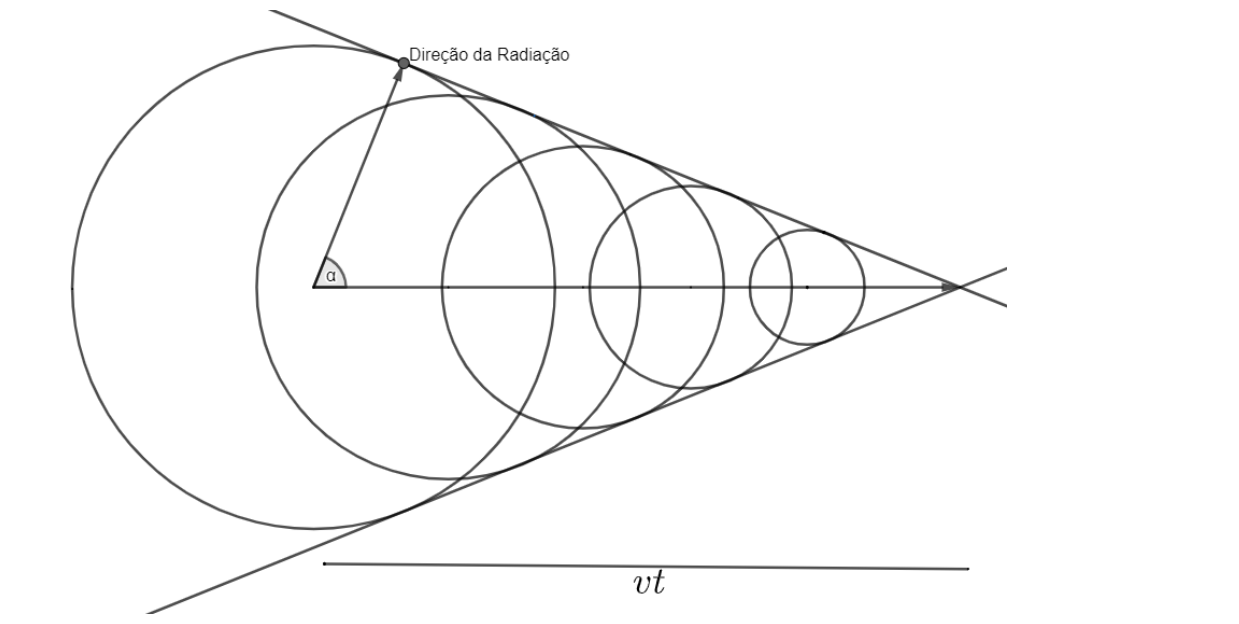
\includegraphics[width=0.9\linewidth]{imagens/cherenkov.png}  
      \caption{Mecanismo de radiação do Efeito Cherenkov}
    \end{figure}

    Esse efeito é similar a um jato movendo-se em velocidade supersônica, ou seja, segue o mesmo
    princípio do Cone de Mach, porém, com a luz. Finalmente, iremos desenvolver o modelo matemático do Efeito Cherenkov.

    \begin{center}
        \textbf{Parte A - Modelo Teórico}    
    \end{center}
    
    Considere uma partícula movimentando-se a velocidades relativísticas em um meio de índice de
    refração $n$. Sabe-se que sua massa de repouso é $m_0$, possui momento linear $p$ e velocidade $v$. Em
    determinado momento, há emissão de um fóton sob um ângulo $\alpha$, como mostra a figura 1.

    \begin{alternativas}
        \item Sendo $\mu$ a frequência do fóton emitido, determine a equação de seu momento
        linear, $p_\mu$, e sua energia, $E_\mu$. Sua resposta deve estar em função de $n$, $\mu$ e constantes físicas.
        \item Encontre uma expressão para o momento linear da partícula após a emissão
    do fóton em função de $p_\mu$, $p$ e $\alpha$.
        \item Sendo $\beta_n = \frac{c}{vn}$, prove que a relação abaixo é verdadeira:
        \begin{equation}
            \cos\alpha = \frac{1}{\beta_n}
        \end{equation}
        \item Considerando que o momento linear e a energia se conservem, determine a
        velocidade mínima para a ocorrência do Efeito Cherenkov.
        \textbf{Dica:} Quando comparado com os outros parâmetros, o fator $(n^2-1)h\mu$ pode ser desprezado.

    \begin{center}
        \textbf{Parte B - Reações Nucleares}    
    \end{center}
    
    A cadeia próton-próton é um processo de reações de fusão para conversão de hidrogênio em hélio.
    Um dos ramos possíveis da cadeia próton-próton é a $pp \text{ IV}$, na qual, teoricamente, um átomo de
    hélio-3 reage diretamente com um próton, conforme a reação a seguir:

    \begin{equation}
        ^3\text{He} + ^1\text{H} \rightarrow ^4\text{He} + \nu + \_\_
    \end{equation}

        \item  Indicando a lei de conservação nuclear utilizada, indique qual partícula faltante
        no quadrado da reação acima.

        \item  Indicando a lei de conservação nuclear utilizada, indique qual partícula faltante
        no quadrado da reação abaixo:

        \begin{equation}
            \pi^- \rightarrow \mu^- + \_
        \end{equation}
        
        \textbf{Dados:} Massa do píon: $140 \ \text{MeV}/c^2$, massa do múon: $106 \ \text{MeV}/c^2$.
    \end{alternativas}

\begin{pssolution*}{}{}
    \begin{center}
        \textbf{Parte A - Modelo Teórico}    
    \end{center}

    \begin{alternativas}
        \item Para um fóton, as relações de De Broglie, nos dizem que 
        \[E = h\mu, \ \ p = \frac{h}{\lambda}\]
        Onde \(h\) é a constante de plank.

        Utilizando a relação fundamental da ondulatória, \(\lambda = v/\mu = \frac{c}{n\mu}\), assim 

        \[\boxed{E = h\mu, \ \ p = \frac{nh\mu}{c}}\]

        \item Como o momento total é conservado, considereque a particula está se movendo com momento \(p\) ao longo do eixo \(x\), antes de emitir um foton. Assim, temos 
        
        \[p = p_\mu\cos\alpha + p'_x\]

        \[p_\mu\sin\alpha = p'_y\]

        \[p' = \sqrt{p_x^2 + p_y^2}\]

        Resolvendo para \(p'\)

        \[p'^2 =(p - p_\mu\cos\alpha)^2 +p_\mu^2\sin^2\alpha \]

        \[p'^2 = p^2 - 2p_\mu p \cos\alpha + p_\mu^2\]

        Finalmente

        \[p' = \sqrt{p^2-2pp_\mu\cos\alpha+p^2_\mu}\]

        \item Olhe a seguinte figura, 
        
        \begin{figure}[H]
            \centering
            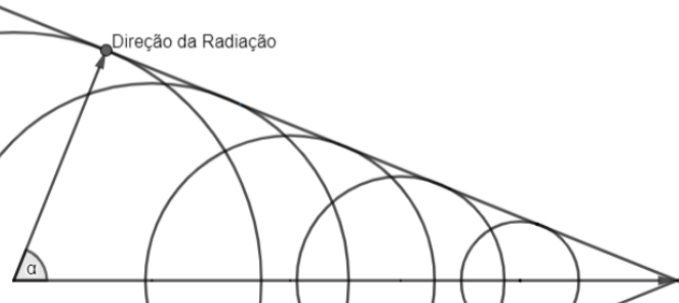
\includegraphics[width=0.7\linewidth]{imagens/cherenkov.1.png}
            \caption{Esquema Cherenkov}
        \end{figure}

        Note que o raio do circulo é dado pela distância percorrida pelo fóton. A distância percorrida do centro do cirulo até o fim do cone é \(vt\), assim

        \[\boxed{\cos\alpha = \frac{ct}{nvt} = \frac{c}{nv} \equiv \frac{1}{\beta_n}}\]

        \item Definindo \(c=1\), a conservação de energia nos diz
        \[\sqrt{p^2+m_0^2} = \sqrt{p'^2+m_0^2}+h\mu\]

        Trablhando nessa expressão

        \[\sqrt{p'^2 + m_0^2} = \sqrt{p^2+m_0^2} - h\mu\]

        \[p'^2 + m_0^2 = p^2+m_0^2 + h^2\mu^2 - 2h\mu\sqrt{p^2+m_0^2}\]

        Substituindo \(p'\)

        \[p^2-2pp_\mu\cos\alpha+p^2_\mu = p^2+h^2\mu^2 - 2h\mu\sqrt{p^2+m_0^2}\]

        Resolvendo para \(\cos\alpha\) 

        \[\cos\alpha = \frac{p_\mu^2 - h^2\mu^2+2h\mu\sqrt{p^2+m_0^2}}{2pp\mu}\]

        Simplificando 

        \[\cos\alpha = \frac{p_\mu}{2p} - \frac{h^2\mu^2}{2pp_\mu} + \frac{h\mu\sqrt{p^2+m_0^2}}{pp_\mu}\]
        
        Substituindo \(p_\mu = nh\mu\)

        \[\cos\alpha = \frac{nh\mu}{2p} + \frac{h\mu}{2np}+ \frac{\sqrt{p^2+m_0^2}}{np}\]

        \[\cos\alpha = \frac{h\mu(n^2-1)+2\sqrt{p^2+m_0^2}}{2np}\]

        Desprezando o termo \(h\mu(n^2-1)\) e substituindo \(\cos\alpha\)

        \[\frac{1}{nv} = \frac{\sqrt{p^2+m_0^2}}{np}\]

        Resolvendo para \(v\)

        \[v = \frac{p}{\sqrt{p^2+m_0^2}}\]

        Porfim, voltando os \(c\)'s, temos 

        \[\boxed{v = \frac{pc^2}{\sqrt{p^2c^2+m_0^2c^4}}}\]

        \begin{center}
            \textbf{Parte B - Reações Nucleares}    
        \end{center}

        \item Utilizando a conservação de carga, do lado esquerdo temos \(2+1=3\) prótons, porém do lado direito, só temos \(2\), portanto a particula faltante deve conter um proton. Já a massa atômica, segue como \(3+1=4\) e do lado direito \(4\). Assim, a particula faltante deve ter a carga de um proton e a massa muito menor do que este. A única partícula que seja essa descrição é o \(\boxed{\text{pósiton, }e^+}\).
            
        \item Utilizando que o número leptônico é constante, temos que o pion não é um lepton \(n_L=0\), mas o múon, é um lepton com \(n_L=+1\), então a nossa partícula deve ter \(n_L=-1\). O únio antilépton neutro associado ao múon com \(n_L=-1\) é o antineutrino do múon, \(\bar{\nu}_\mu\), portanto, a relação completa é 
        \[\boxed{\pi^{-}\rightarrow \mu^- + \bar{\nu}_\mu}{}\]

    \end{alternativas}

\end{pssolution*}
\end{pproblem}


\pts{3} 
\begin{pproblem}(Lista 3 - Vinhedo 2022)
Juvelino, diretamente de seu observatório em Paris, França, monitora a estrela Polaris ($\alpha\text{UMi}$). Ele tem como objetivo descobrir a temperatura de cor $T_c$ do astro. Alguns dos dados de que ele dispõe a respeito de seu alvo são:

\begin{itemize}
    \item Magnitude aparente na banda $V$: $V = 1,98$;
    \item Magnitude absoluta na banda $V$: $M_V = -3,60$;
    \item Magnitude absoluta na banda $B$: $M_B = -3,19$.
\end{itemize}

Com as informações fornecidas, ajude Juvelino!

\begin{alternativas}
    \item Realizando diversas observações, Juvelino determinou que a extinção interestelar na banda $V$ na direção de Polaris é $a_V = 5,8 \, \text{mag/kpc}$. Determine a distância, em pc, de $\alpha\text{UMi}$ até a Terra.
    \item Usando a relação empírica
    \begin{equation}
        \frac{A_V}{E_{B-V}} = 3,0
    \end{equation}
    sendo $A_V$ a extinção interestelar total na banda $V$ e $E_{B-V}$ o excesso de cor $B-V$, determine o índice de cor $B-V$ da estrela observada.
    \item Demonstre a relação
    \begin{equation}
        T_c = \frac{7009}{(B-V) + 0,47}
    \end{equation}
    na qual a temperatura de cor é dada em Kelvin. Para tanto, use o fato de que estrelas de classe espectral $A0$ possuem $(B-V) = 0$ e $T_c = 15000 \, \text{K}$. Use também que os comprimentos de onda das bandas $B$ e $V$ são, respectivamente, $\lambda_B = 440 \, \text{nm}$ e $\lambda_V = 548 \, \text{nm}$. Justifique quaisquer aproximações feitas.

    \textbf{DICA: A lei de plack talvez seja útil}
    \item Determine a temperatura de cor de Polaris.
\end{alternativas}
\begin{pssolution*}{}{}
    \begin{alternativas}
        \item A expressão que relaciona corretamente as magnitudes é 
        \[V - M_V = 5 \log d - 5 + a_V d\]

        Essa equação, só pode ser resolvida por meio da iteração,

        \[d = \frac{V-M_V - 5\log d + 5}{a_v}\]

        Iterando, chegamos em \(\boxed{d\approx 100\text{ pc}}\).

        \item Pela definição, \(E_{B-V} = A_B - A_V\). Assim
        
        \[\frac{A_V}{A_B-A_V} = 3,00\]

        \[A_B = \frac{A_V}{3}+A_V = 0,77\]

        Assim, 

        \[B-M_B = 5\log d - 5 + A_B\rightarrow B = 2,58\]

        E pela definição, o índice \(B-V\) = \(\boxed{U_{B-V} = B-V = 0,60}\)

        \item Utilizando a Lei de Planck, temos que 
        
        \[\frac{B_B}{B_V} = \frac{F_B}{F_V} \left(\frac{\lambda_V}{\lambda_B}\right)^5 \frac{e^{\frac{\beta hc}{\lambda_V}-1}}{e^{\frac{\beta hc}{\lambda_B}-1}}\]

        Utilizando a aproximação de Wein, temos

        \[\frac{F_B}{F_V} = \left(\frac{\lambda_V}{\lambda_B}\right)^5 \frac{e^{\frac{\beta hc}{\lambda_V}}}{e^{\frac{\beta hc}{\lambda_B}}}\]

        Utilizando a equação de Pogson para comparar as magnitudes, 

        \[B-V = -2,5\log\left(\frac{F_B}{F_V}\right)+C\]

        Aqui adicionamos uma constante, pois estamos trabalhando com diferentes comprimentos de ondas. Trabalhando na expressão, 

        \[B-V = -2,5\log\left(\left(\frac{\lambda_V}{\lambda_B}\right)^5 \frac{e^{\frac{\beta hc}{\lambda_V}}}{e^{\frac{\beta hc}{\lambda_B}}}\right)+C\]

        Trabalhando nessa expressão, 

        \[B-V = -2,5\log\left(\frac{\lambda_V}{\lambda_B}\right)^5 + 2,5 \beta hc\left(\frac{1}{\lambda_B}-\frac{1}{\lambda_V}\right)\log e + C\]

        E utilizando \(\beta = \frac{1}{k_B T_c}\) e substituindo os valores, 

        \[B-V = -1,19 + \frac{7009}{T_c}+C\]

        Para o tipo \(A_0\), \((B_V)=0\) e \(T_c = 15000\)K. Assim, 

        \[-1,19 + \frac{7009}{15000} + C = 0 \rightarrow C = 0,72\]

        Assim, 

        \[B-V = -0,47 + \frac{7009}{T_c} \rightarrow \ \ \boxed{T_c = \frac{7009}{(B-V) + 0,47}}\]

        \item da equação anterior, 
        
        \[\boxed{T_c = \frac{7009}{0,60 + 0,47} \approx 6600 \text{ K}}\]
    \end{alternativas}    

\end{pssolution*}
\end{pproblem}


\pts{4}
\begin{pproblem}
    (Lista 4 - 2020) Apesar de assustadora, a plantação de bananeiras de Juvelino possui um céu perfeito para uma de suas duas paixões: astrofotografia. Ele possui um telescópio de 200 mm de diâmetro e uma super CCD acoplada, com os parâmetros: lado do pixel \(5\ \mu\text{m}\), escala de placa \(3,2\ \text{arcmin/mm}\), eficiência quântica de 97\%, RON (Read-out noise, ou ruído de leitura) 1 contagem/pixel e DN (ruído térmico) 1 contagem/(pixel.hora). Ele prefere fazer suas observações na banda \(V\) (comprimento de onda central \(\lambda_V = 5500\ \text{Å}\), largura de banda \(\Delta \lambda = 820\ \text{Å}\)), pois lembra-se de um número mágico associado a ela: o fluxo de fótons de um objeto de magnitude 0 nessa banda é \(\phi_0 = 1000\ \text{fótons/}(\AA\cdot \text{cm}^2)\). Juvelino possui 2 alvos prediletos: uma estrela de magnitude \(m_V = 4,51\) e um aglomerado globular de brilho superficial uniforme em \(V\) de \(19,5\ \text{mag/arcsec}^2\) e diâmetro angular \(\theta = 40''\).
\end{pproblem}


\end{document}